% Options for packages loaded elsewhere
\PassOptionsToPackage{unicode}{hyperref}
\PassOptionsToPackage{hyphens}{url}
\PassOptionsToPackage{dvipsnames,svgnames,x11names}{xcolor}
%
\documentclass[
  letterpaper,
  DIV=11,
  numbers=noendperiod]{scrreport}

\usepackage{amsmath,amssymb}
\usepackage{lmodern}
\usepackage{iftex}
\ifPDFTeX
  \usepackage[T1]{fontenc}
  \usepackage[utf8]{inputenc}
  \usepackage{textcomp} % provide euro and other symbols
\else % if luatex or xetex
  \usepackage{unicode-math}
  \defaultfontfeatures{Scale=MatchLowercase}
  \defaultfontfeatures[\rmfamily]{Ligatures=TeX,Scale=1}
\fi
% Use upquote if available, for straight quotes in verbatim environments
\IfFileExists{upquote.sty}{\usepackage{upquote}}{}
\IfFileExists{microtype.sty}{% use microtype if available
  \usepackage[]{microtype}
  \UseMicrotypeSet[protrusion]{basicmath} % disable protrusion for tt fonts
}{}
\makeatletter
\@ifundefined{KOMAClassName}{% if non-KOMA class
  \IfFileExists{parskip.sty}{%
    \usepackage{parskip}
  }{% else
    \setlength{\parindent}{0pt}
    \setlength{\parskip}{6pt plus 2pt minus 1pt}}
}{% if KOMA class
  \KOMAoptions{parskip=half}}
\makeatother
\usepackage{xcolor}
\setlength{\emergencystretch}{3em} % prevent overfull lines
\setcounter{secnumdepth}{5}
% Make \paragraph and \subparagraph free-standing
\ifx\paragraph\undefined\else
  \let\oldparagraph\paragraph
  \renewcommand{\paragraph}[1]{\oldparagraph{#1}\mbox{}}
\fi
\ifx\subparagraph\undefined\else
  \let\oldsubparagraph\subparagraph
  \renewcommand{\subparagraph}[1]{\oldsubparagraph{#1}\mbox{}}
\fi


\providecommand{\tightlist}{%
  \setlength{\itemsep}{0pt}\setlength{\parskip}{0pt}}\usepackage{longtable,booktabs,array}
\usepackage{calc} % for calculating minipage widths
% Correct order of tables after \paragraph or \subparagraph
\usepackage{etoolbox}
\makeatletter
\patchcmd\longtable{\par}{\if@noskipsec\mbox{}\fi\par}{}{}
\makeatother
% Allow footnotes in longtable head/foot
\IfFileExists{footnotehyper.sty}{\usepackage{footnotehyper}}{\usepackage{footnote}}
\makesavenoteenv{longtable}
\usepackage{graphicx}
\makeatletter
\def\maxwidth{\ifdim\Gin@nat@width>\linewidth\linewidth\else\Gin@nat@width\fi}
\def\maxheight{\ifdim\Gin@nat@height>\textheight\textheight\else\Gin@nat@height\fi}
\makeatother
% Scale images if necessary, so that they will not overflow the page
% margins by default, and it is still possible to overwrite the defaults
% using explicit options in \includegraphics[width, height, ...]{}
\setkeys{Gin}{width=\maxwidth,height=\maxheight,keepaspectratio}
% Set default figure placement to htbp
\makeatletter
\def\fps@figure{htbp}
\makeatother
\newlength{\cslhangindent}
\setlength{\cslhangindent}{1.5em}
\newlength{\csllabelwidth}
\setlength{\csllabelwidth}{3em}
\newlength{\cslentryspacingunit} % times entry-spacing
\setlength{\cslentryspacingunit}{\parskip}
\newenvironment{CSLReferences}[2] % #1 hanging-ident, #2 entry spacing
 {% don't indent paragraphs
  \setlength{\parindent}{0pt}
  % turn on hanging indent if param 1 is 1
  \ifodd #1
  \let\oldpar\par
  \def\par{\hangindent=\cslhangindent\oldpar}
  \fi
  % set entry spacing
  \setlength{\parskip}{#2\cslentryspacingunit}
 }%
 {}
\usepackage{calc}
\newcommand{\CSLBlock}[1]{#1\hfill\break}
\newcommand{\CSLLeftMargin}[1]{\parbox[t]{\csllabelwidth}{#1}}
\newcommand{\CSLRightInline}[1]{\parbox[t]{\linewidth - \csllabelwidth}{#1}\break}
\newcommand{\CSLIndent}[1]{\hspace{\cslhangindent}#1}

\KOMAoption{captions}{tableheading}
%\usepackage{setspace}
%\onehalfspacing
%\doublespacing
%\usepackage{arxiv}
\makeatletter
\makeatother
\makeatletter
\@ifpackageloaded{bookmark}{}{\usepackage{bookmark}}
\makeatother
\makeatletter
\@ifpackageloaded{caption}{}{\usepackage{caption}}
\AtBeginDocument{%
\ifdefined\contentsname
  \renewcommand*\contentsname{Table of contents}
\else
  \newcommand\contentsname{Table of contents}
\fi
\ifdefined\listfigurename
  \renewcommand*\listfigurename{List of Figures}
\else
  \newcommand\listfigurename{List of Figures}
\fi
\ifdefined\listtablename
  \renewcommand*\listtablename{List of Tables}
\else
  \newcommand\listtablename{List of Tables}
\fi
\ifdefined\figurename
  \renewcommand*\figurename{Figure}
\else
  \newcommand\figurename{Figure}
\fi
\ifdefined\tablename
  \renewcommand*\tablename{Table}
\else
  \newcommand\tablename{Table}
\fi
}
\@ifpackageloaded{float}{}{\usepackage{float}}
\floatstyle{ruled}
\@ifundefined{c@chapter}{\newfloat{codelisting}{h}{lop}}{\newfloat{codelisting}{h}{lop}[chapter]}
\floatname{codelisting}{Listing}
\newcommand*\listoflistings{\listof{codelisting}{List of Listings}}
\makeatother
\makeatletter
\@ifpackageloaded{caption}{}{\usepackage{caption}}
\@ifpackageloaded{subcaption}{}{\usepackage{subcaption}}
\makeatother
\makeatletter
\@ifpackageloaded{tcolorbox}{}{\usepackage[many]{tcolorbox}}
\makeatother
\makeatletter
\@ifundefined{shadecolor}{\definecolor{shadecolor}{rgb}{.97, .97, .97}}
\makeatother
\makeatletter
\makeatother
\ifLuaTeX
  \usepackage{selnolig}  % disable illegal ligatures
\fi
\IfFileExists{bookmark.sty}{\usepackage{bookmark}}{\usepackage{hyperref}}
\IfFileExists{xurl.sty}{\usepackage{xurl}}{} % add URL line breaks if available
\urlstyle{same} % disable monospaced font for URLs
\hypersetup{
  pdftitle={Analysis Demos},
  colorlinks=true,
  linkcolor={blue},
  filecolor={Maroon},
  citecolor={Blue},
  urlcolor={Blue},
  pdfcreator={LaTeX via pandoc}}

\title{Analysis Demos}
\author{Jordan B. Gunn\\
Cognition and Cognitive Neuroscience Program\\
Vanderbilt University\\
Nashville, TN 37235\\
\texttt{jordan.gunn@vanderbilt.edu} \and \textbf{Sean M. Polyn}\\
Department of Psychological Sciences\\
Vanderbilt University\\
Nashville, TN 37235\\
\texttt{sean.polyn@vanderbilt.edu}}
\date{}

\begin{document}
\maketitle
\ifdefined\Shaded\renewenvironment{Shaded}{\begin{tcolorbox}[interior hidden, sharp corners, enhanced, borderline west={3pt}{0pt}{shadecolor}, breakable, frame hidden, boxrule=0pt]}{\end{tcolorbox}}\fi

\bookmarksetup{startatroot}

\hypertarget{section}{%
\chapter{}\label{section}}

Demonstrations of analysis supported by my compmemlearn library.

\bookmarksetup{startatroot}

\hypertarget{the-serial-position-effect}{%
\chapter{The Serial Position Effect}\label{the-serial-position-effect}}

The serial position effect describes how our memory is affected by the
position of information in a sequence or list. Research tends to find
that people best remember the first and last items in a series and find
it hard to remember the middle items. To measure the serial position
effect, research participants perform a free recall task where they
study a list of items and subsequently ``freely'' recall the items in
the order in which they come to mind. The recall rate of each item at
each study position across these lists reflects the serial position
effect.

\begin{figure}

{\centering 

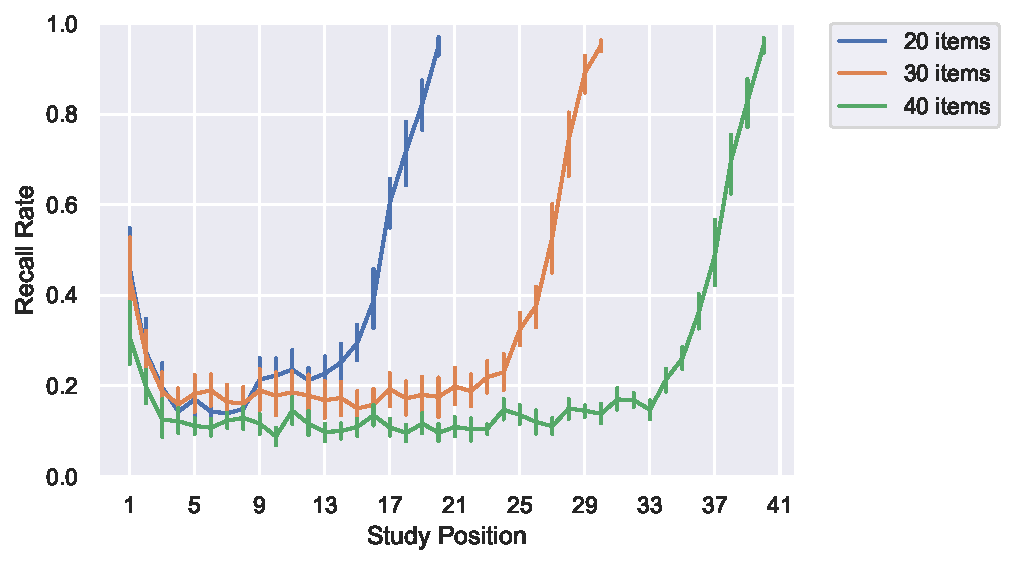
\includegraphics{analyses/figures/Murdock1962_spc.pdf}

}

\caption{\label{fig-Murdock1962_spc}The serial position effect measured
as a function of list length using data from Murdock Jr (1962).}

\end{figure}

\bookmarksetup{startatroot}

\hypertarget{the-lag-contiguity-effect}{%
\chapter{The Lag-Contiguity Effect}\label{the-lag-contiguity-effect}}

The lag-contiguity effect illustrates how episodic associations are
graded, exhibiting power-function decay with increasing lag. Recall of
an item has a tendency to evoke not only adjacent list items, but other
nearby items as well. In addition, episodic associations appear to be
asymmetrical, favoring retrieval of items in the forward order.

The lag-CRP analysis measures the lag-contiguity effect in free recall
data by tracking the conditional probability of retrieving an unrecalled
item as a function of its lag in the study list from the last recalled
item. For example, if a research participant recalls the third item
presented in a list and then the fourth, the corresponding lag is +1. If
a participant instead recalls the first item after recalling the third
item, the measured lag is -2. The ratio of actual divided by possible
lag transitions across a dataset over a range of lag values tends to
identify a lag-contiguity effect.

\begin{figure}

{\centering 

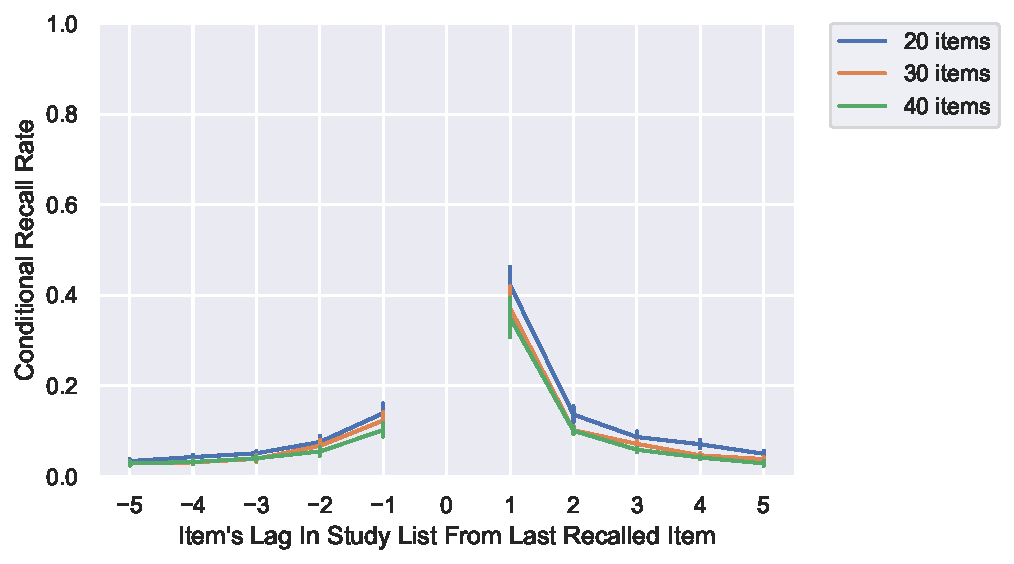
\includegraphics{analyses/figures/Murdock1962_crp.pdf}

}

\caption{\label{fig-Murdock1962_crp}The lag-contiguity effect measured
as a function of list length using data from Murdock Jr (1962) and the
lag-CRP analysis.}

\end{figure}

\bookmarksetup{startatroot}

\hypertarget{probability-of-first-recall}{%
\chapter{Probability of First
Recall}\label{probability-of-first-recall}}

The probability of starting free recall with the item at each position
in a studied sequence or list.

\begin{figure}

{\centering 

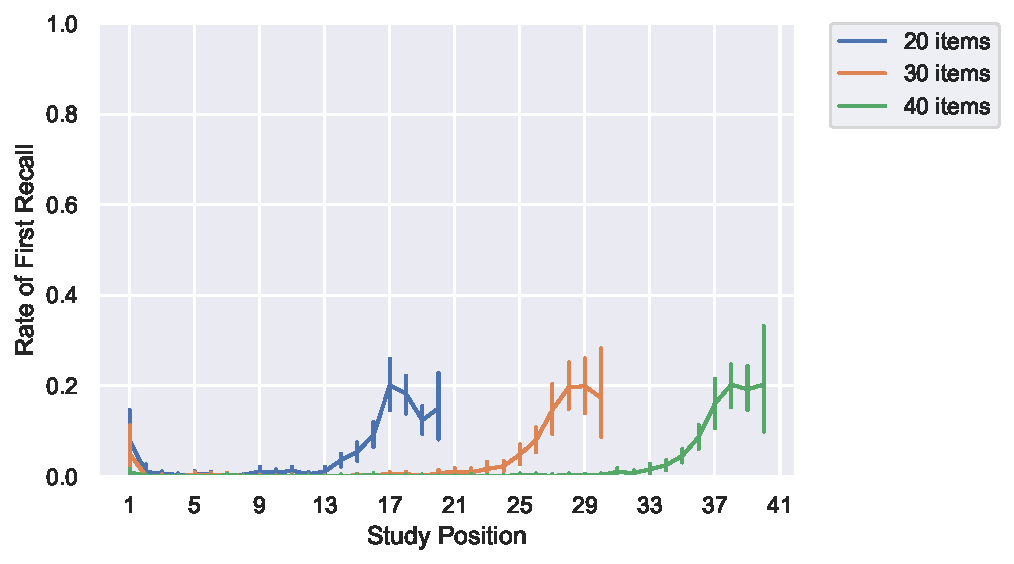
\includegraphics{analyses/figures/Murdock1962_pfr.pdf}

}

\caption{\label{fig-Murdock1962_pfr}Rate of first recall by serial
position measured as a function of list length using data from Murdock
Jr (1962).}

\end{figure}

\bookmarksetup{startatroot}

\hypertarget{references}{%
\chapter{References}\label{references}}

\hypertarget{refs}{}
\begin{CSLReferences}{1}{0}
\leavevmode\vadjust pre{\hypertarget{ref-murdock1962serial}{}}%
Murdock Jr, B. B. (1962). The serial position effect of free recall.
\emph{Journal of Experimental Psychology}, \emph{64}(5), 482.

\end{CSLReferences}



\end{document}
